%\subsection{Effect of lens radius}
%lensed_waveguide_radium
In this part the effect of the radius of the lens interface of the lensed waveguide will be discussed. Coupling simulations of 3 groups are arranged and the lens height is kept as a constant of $1\mu$m, $1.5\mu$m and $2\mu$m, respectively.  The distance of the waveguide end face from TLF maintains $4\mu$m and the lens radius of the lensed waveguide is varied from $2\mu$m to $3\mu$m with step of $02\mu$m.\\
 
\begin{table}[!ht]
\caption{Coupling efficiency between TLF and lensed waveguide due to changing the lens radius.}
\centering
\begin{tabular}{|c|c|c|c|}
\hline
\multirow{2}*{Radius($\mu$m)}&\multicolumn{3}{c|}{Height($\mu$m)}\\
\cline{2-4}
 								&	1&	1.5&2\\
\hline
$2.0$& $59.5\%$	&$61.3\%$	&$69\%$\\
$2.2$& $59\%$		&$60.8\%$	&$68.3\%$\\
$2.4$&$59\%$		&$60.3\%$	&$66.8\%$\\
$2.6$&$58.6\%$	&$59.9\%$	&$65.3\%$\\
$2.8$&$58.2\%$	&$59.3\%$	&$64\%$\\
$3.0$&$57.8\%$	&$58.7\%$	&$63\%$\\
\hline
\end{tabular}
\label{tab:coupling_lensed_waveguide_radium}
\end{table}
\begin{figure}[!ht]
\centering
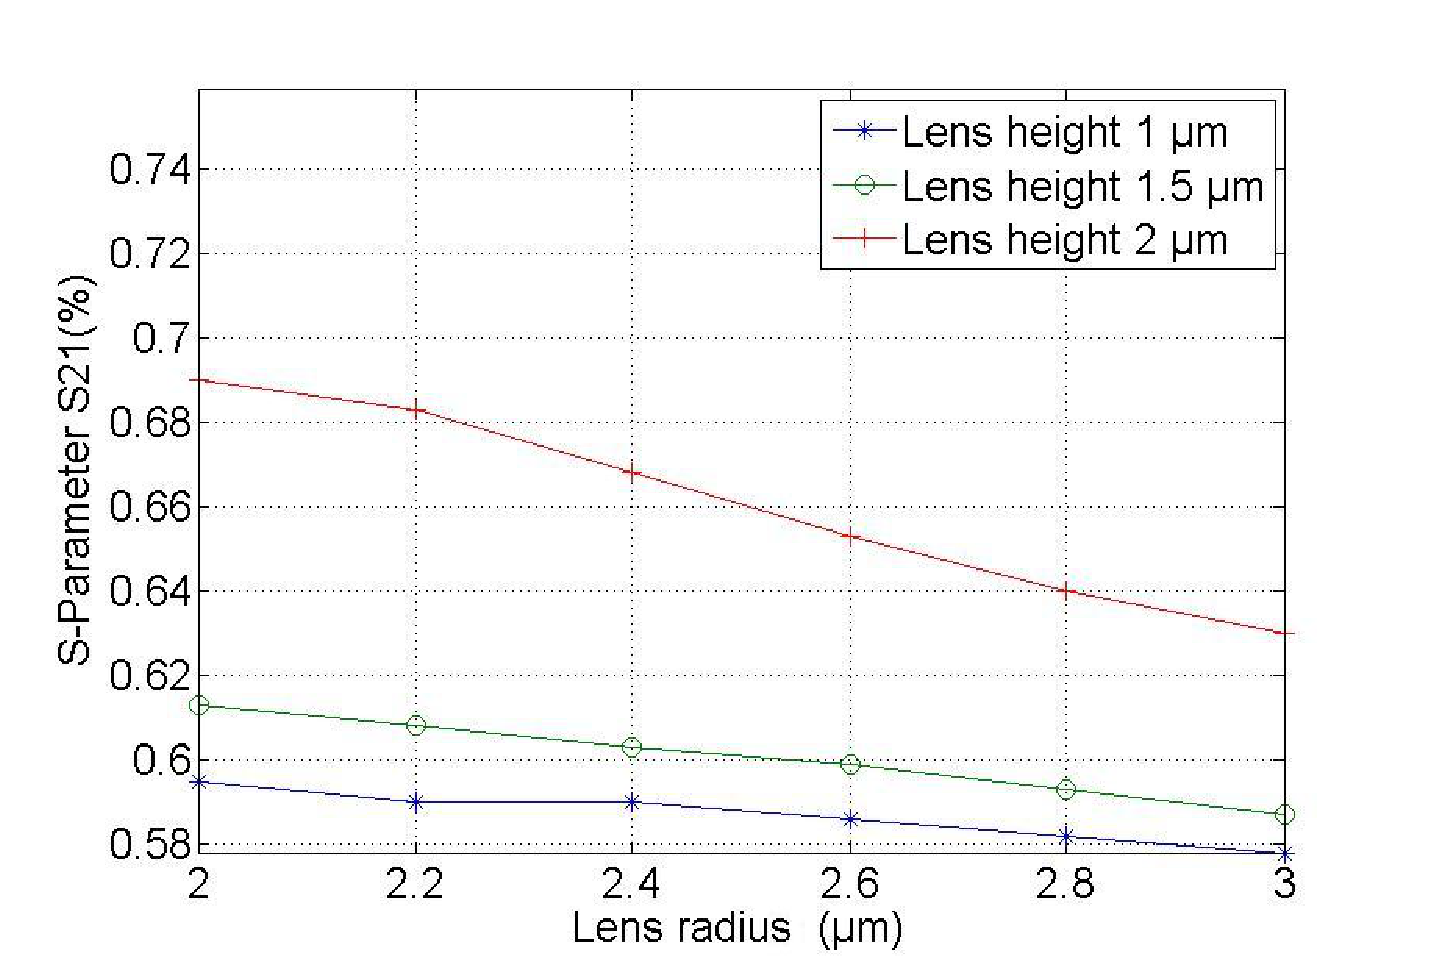
\includegraphics[width=0.8\textwidth]{bilder/s21_fix_lens_height_rxx}
\caption{Coupling efficiency due to changing the lens radius.}
\label{fig:coupling_lenses_curve_rxx}
\end{figure}
Tab. \ref{tab:coupling_lensed_waveguide_radium} demonstrates coupling results of these arrangements and Fig. \ref{fig:coupling_lenses_curve_rxx} exhibits their coupling behaviors with the lens radius increasing. Apparently, it can be told that the coupling efficiency of each group is monotonously declining due to the variation of the lens radius. For the smallest radius value of $2\mu$m the coupling efficiency has the maximal values, $59.5\%$ for $h'=1\mu$m, $61.3\%$ for $h'=1.5\mu$m, $69\%$ for $h'=2\mu$m. For the maximal radius value of $3\mu$m the coupling efficiency has the minimum values, $57.8\%$ for $h'=1\mu$m, $58.7\%$ for $h'=1.5\mu$m, $63\%$ for $h'=2\mu$m.\\

\begin{figure}[!ht]
\centering
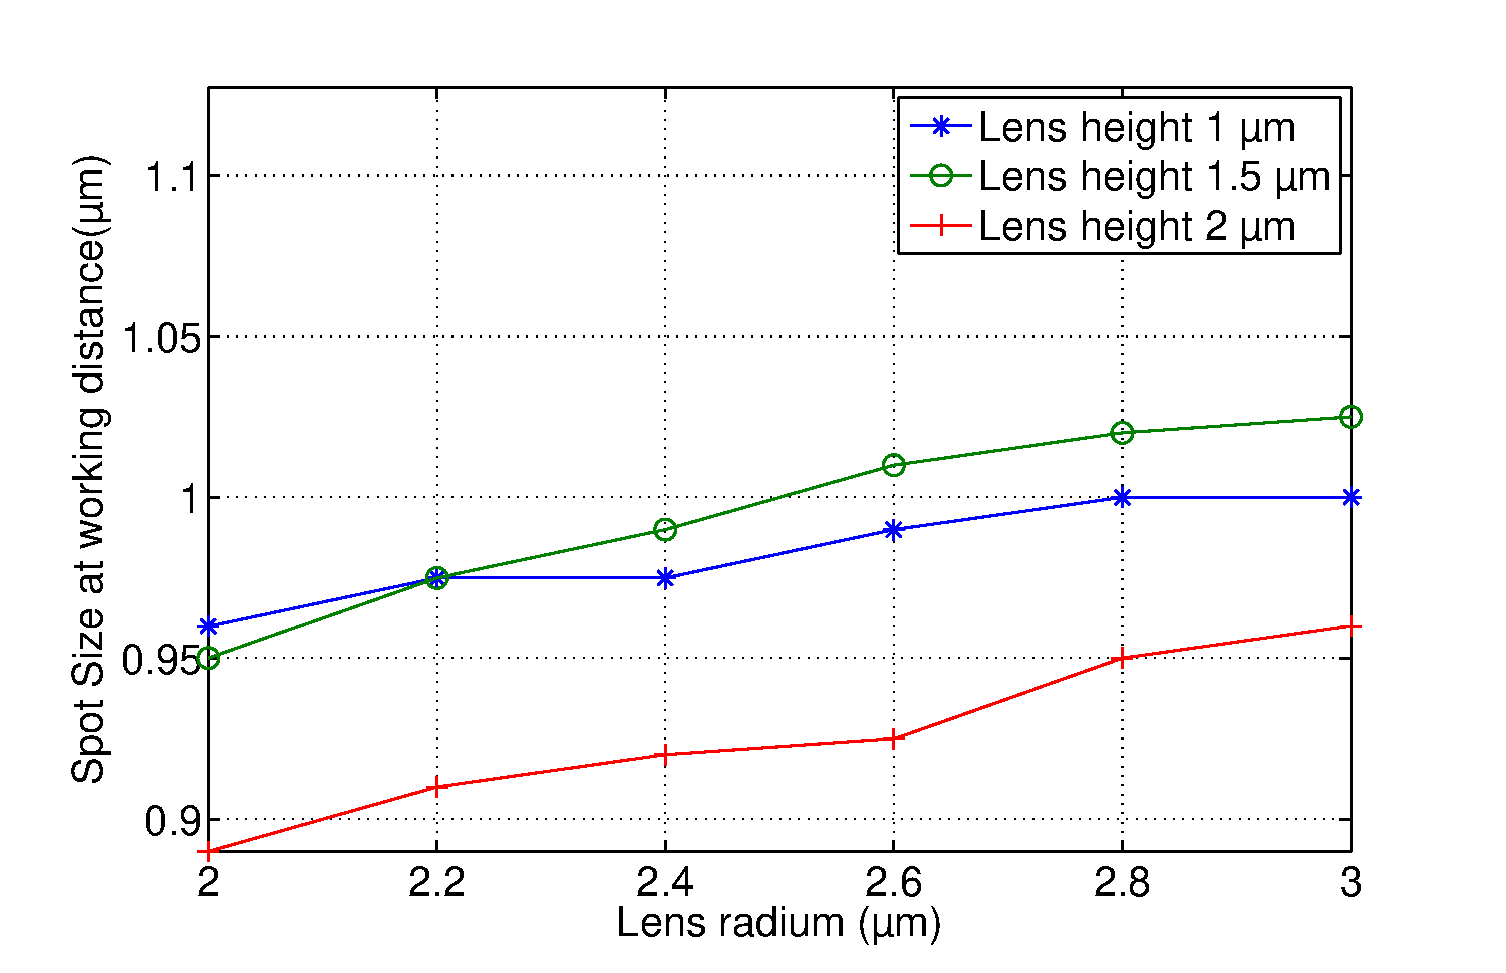
\includegraphics[width=0.7\textwidth]{bilder/spot_fix_lens_height_rxx}
\caption{The spot size curve at lensed waveguide interface due to changing lens height.}
\label{fig:lensed_guide_spot_size_curve_rxx}
\end{figure}
As previous Section \ref{sect:optim_lensed_height} the tendency in Fig. \ref{fig:coupling_lenses_curve_rxx} can be verified by their spot size curve in Fig. \ref{fig:lensed_guide_spot_size_curve_rxx}. The spot size curve of each group behaves along the variation of the lens radius inversely in compare with the trends of coupling efficiency. 

%\Subsection{Conclusions of lensed waveguide}
 According previous discussion about lensed waveguides following conclusions can be given: 
\begin{itemize} 
\item The coupling efficiency of Fiber-to-Chip can be significantly improved by applying lensed waveguides.  
\item The coupling efficiency of lensed waveguide is rising with the lens height increasing and the lens radius decreasing.
\item The optimal design of lensed waveguides is a hemisphere lens structure. 
\end{itemize}
